% !TEX root = ../CSS-OS.tex

\chapter{工作日志}

{\heiti 这一章主要记录与詹老师和张鑫的讨论的过程中所产生的一些想法,以及每天相应的工作日志。}

%%%%%%%%%%%%%%%%%%%%%%%%%%%%%%%%%%%%%%%%%%%%%%%%%%%%%%%%%%%%%%%%%%%
\section{3月}
\subsection{16日}

\subsubsection{本次讨论提到的主要内容}

\begin{itemize}
\item {\textbf{两种明显的非优化的情况}}\\
1. 当望远镜处于某个有很多可观测天区的位置时,那些可观测天区早已经被观测完,导致望远镜进入
等待状态,因此会浪费掉很多的观测时间。如果出现这样的情况,也许可以考虑观测某些未事先纳入
观测范围的天区,例如黄道夹角20°附近的边缘区域。

2. 由于规划策略不合理,导致望远镜进入观测死角,比如要转向下一个可观测天区时需要进行大角度的
转动(这种情况不是不允许,而是如果经常出现这样情况的话,一定程度上说明了规划的观测序列不是
很合理,因为大角度的转动比较的费时,且更加不容易满足各项条件的限制。

\item {\textbf{量化优化}}\\
首先有两个概念需要明确。一是有效观测时间,可以粗略的理解为10年内的曝光时间(增加曝光面积)
的总和;二是可观测时间,可粗略的理解为10年的总时间扣除掉那些由于“硬性条件”(如SAA区域、
平台转动、地球遮挡等)所不能观测的时间(这个时间可以根据模拟的结果进行统计)。那么可以将
优化效率定义为:
\begin{eqnarray}
\text{优化效率} = \frac{\text{有效观测时间}}{\text{可观测时间}}.
\end{eqnarray}
显然,此处定义的效率的计算是依赖于具体的模拟结果的。

\item {\textbf{对“一轨”的理解}}\\
目前的模拟程序每一步的判断都是基于对“一轨”的限制条件来进行的。但是前后两次“一轨”的交叉部分
也可以看作是“一轨”,那么对这个“一轨”所需要满足的条件该如何判断?目前的代码还没有考虑这个问题。

\item {\textbf{权重}}\\
所提引进的各项权重是应该“相加”还是“相乘”?这个问题的答案似乎只能是依靠多次模拟的结果来进行判断了。

\item {\textbf{对未来模拟程序功能上的一些预期}}\\
目前的模拟是假设所有的观测是按部就班地进行的,即所有的观测都是事先编排好了的,中途不会出现
突发情况,例如在某个时期需要将望远镜对准某些区域进行一些特殊用途的观测。而实际观测中肯定会
出现一些特殊的需求,因此新的模拟程序需要能够处理这些特殊需求。简单说就是可以将这些特殊的需
求作为一种输入“告诉给”模拟程序,然后程序迅速地进行模拟,从而确定这样的特殊需求是否可以做到,
并且不会影响整体的宇宙学观测任务的实施。

\subsubsection{目前的主要任务}
目前的模拟仍处于初级阶段,各种观测条件的假设还比较的粗略。现阶段的主要问题是\RT{增加能源平衡
条件以及CMG之后,模拟结果显示10年内能够观测到的天区面积比预期的要小不少}。因此目前的最重要
的任务是找到使得观测天区面积减少的原因。


\subsubsection{\textbf{逆向工程(Reverse Engineering)}}
如果某些给定的限制条件给得比较粗糙(有一些细节未披露),而我们觉得可以比较物理地去优化这些
条件,那么可以利用逆向工程的方法。我们根据合理的假设进行推演从而得出“限制条件”,然后将这些条
件与那些给定的条件进行对比。如果我们推演得到的条件与给定的条件一致或者非常接近,那么就可以
利用这个条件的“物理模型”去进行模拟(原先的条件通常是一些离散的条件,因此在代码从需要一系列的
判断语句,效率上有一定的折扣);如果存在明显的差异,那就进行适当的模型修改等等,尽可能地
找到原来那些条件的一个比较物理的描述。

\end{itemize}

%%%%%%%%%%%%%%%%%%%%%%%%%%%%%%%%%%%%%%%%%%%%%%%%%%%%%%%%%%%%%%%%%%%
\subsection{19日}
老詹建议可以人为地构造两个“概率分布函数”,用来限制出现两种极端的情况。这两个极端的情况分别
是:1)很快将能源耗尽,也就是在初期的时候,尤其是在阳照区的时候,过多地进行了观测(于是导
致发电不足);2)过分地节约了阳照区的观测机会,即过少地进行了观测,尽管可以节约能源(若减少
观测,则会增加发电的时间),但是浪费掉了观测机会,最终可能导致在规定的巡天时间内无法完成
预期的巡天任务。

\MT{可是这样两个“概率分布函数”该如何定义呢?该选取那些因素作为分布函数的变量呢?}

实际上影响的编排结果的因素有很多,不仅仅上面所提到的两个“概率分布函数”。这次讨论中提到了
“收益”这个概念,可以大致理解为对有效观测面积的增加(可进一步细分)。在某些情况下,比如往某
个指向转动后,能源条件有一定的概率出现不满足,那么是否会继续转动到那个角度去进行观测?在这
个情况下就得根据“收益”来判断,如果没什么收益,那么久没有必要去观测了,反之就可以继续观测。

%%%%%%%%%%%%%%%%%%%%%%%%%%%%%%%%%%%%%%%%%%%%%%%%%%%%%%%%%%%%%%%%%%%
\subsection{21日}

\begin{figure}
\centering
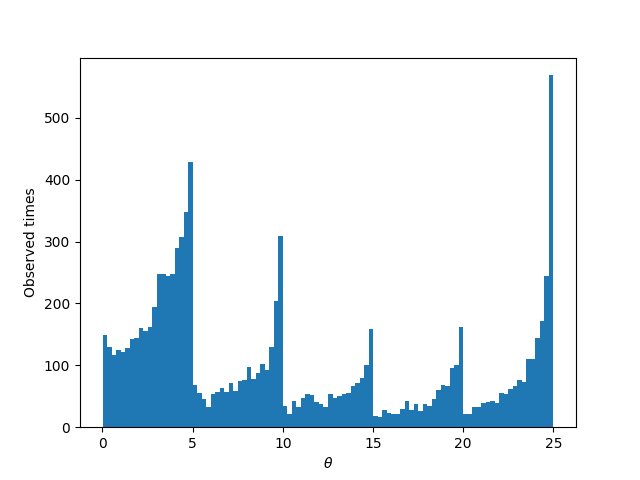
\includegraphics[width=0.7\textwidth]{figs/check_log/fig_0.png}
\caption{帆板法线与太阳的夹角的分布。该图所显示的结果对应于开始观测的最初约146天;后续的
不同时期内的观测情况所对应的统计结果大致与此图所展示的类似。}
\label{0321_hist1d}
\end{figure}

\begin{figure}
\centering
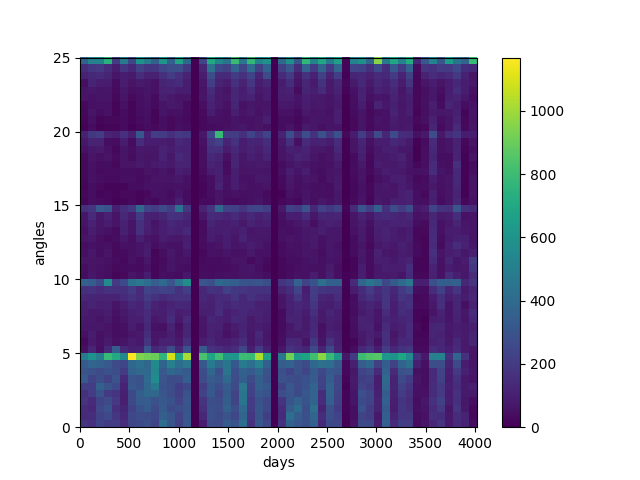
\includegraphics[width=0.75\textwidth]{figs/check_log/time_angle_hist2d.png}
\caption{阳照区的观测次数随观测时间(横轴)以及帆板的法线与太阳夹角(纵轴)的二维直方图分布。}
\label{0321_hist2d_A}
\end{figure}


\begin{figure}
\centering
\includegraphics[width=0.75\textwidth]{figs/check_log/time_trans_angle}
\caption{阳照区的观测次数随观测时间(横轴)以及转动角度的二维直方图分布。}
\label{0321_hist2d_B}
\end{figure}

今天根据张鑫前阵子跑出来的结果进行了简单的分析,统计了一下当望远镜处于阳照区的时候,帆板与
太阳之前夹角的分布情况,统计结果大致如图~\ref{0321_hist1d}和图~\ref{0321_hist2d_A}所示。
3月19日与詹老师讨论的时候,他提到一个预期,那就是平均而言在不同时期内,在阳照区的观测中,
帆板法线与太阳夹角的分布应该是比较平均的(不过我有点怀疑这样一个预期是否有一定的道理,毕竟
我们并不知道最优的编排应该是什么样子的)。图~\ref{0321_hist1d}统计了观测的最初约146天内的
夹角的分布,从中可以看到一些明显有些奇怪的分布:\MT{\textbf{在每一个小的角度区间内,那些大
角度的观测次数明显多于小角度的观测。}}可以看到,这种分布的不均匀性似乎与代码中具体的实现方
式存在一定的联系:每一个小的角度区间内,观测次数最多的总是集中在这个区间的“上界”!

\GT{\heiti 如果我们将这个代码实现进行一下修改,比如从5个区间扩展到10个区间,会不会使得这个
分布变得平缓或者平均一些?}\BT{\kaishu 将张鑫原先的代码从循环判断改为插值如何?如果改为插值
的方式,那么这些插值点如何选择?这里应该需要引入一定的(物理)模型的假设!(添加于3月25日)}



%%%%%%%%%%%%%%%%%%%%%%%%%%%%%%%%%%%%%%%%%%%%%%%%%%%%%%%%%%%%%%%%%%%
\subsection{22日}
今天在读用于获取“进入、离开”阴影区域的时间的函数时,看到其中的一个“步进时间间隔”为60秒,个人
觉得此处可以有优化的余地。为何说有优化的余地呢?主要原因是,这个函数里需要频繁的获取望远镜和
太阳的位置,计算量稍微有点大,需要从预先计算好的轨道数据进行插值,并且望远镜的位置还是事先
(平均)划分到50个字文件中的(程序在进行模拟的时候,这50组数据时存储在50个数组中的),因此
会比较的费时,这就使得步进的时间间隔不能太小。如果在此处改进位置获取的函数,那么就可以用更小
的步进时间来搜索“进入、离开”阴影区域的时间了。

不过首先得确认一个事实,就是60秒的步进间隔是否合理?如果不合理并且确实对编排有一定的影响,
那么就需要从已有的模拟结果中找出一些证据来。

\RT{\textbf{\heiti \sout{那么问题来了,这样的影响会是什么样的?}}}

%%%%%%%%%%%%%%%%%%%%%%%%%%%%%%%%%%%%%%%%%%%%%%%%%%%%%%%%%%%%%%%%%%%
\subsection{23日}
\BT{中午在去711买饭的路上思考(其实是大概估计)了一下这个60秒(\sout{10秒})可能的影响,
发现应该不会有什么大的影响,原因是60秒(\sout{10秒})相对于一轨的92分钟来说,实在是微不足道。}
\RT{\heiti{所以暂时不从这里下手去寻找问题的突破口了。}}


%%%%%%%%%%%%%%%%%%%%%%%%%%%%%%%%%%%%%%%%%%%%%%%%%%%%%%%%%%%%%%%%%%%
\subsection{26日}
今日上午对每次观测时所需要的转动角度进行了统计。具体统计的是为了得到某一个时期内、某个转动
角度范围内的观测次数,结果显示在图~\ref{0321_hist2d_B}中。\BT{\kaishu 从该图可以看到,在绝
大部分的观测时期内,小角度的转动总是占绝大多数的。不过还是可以看出一些不怎么符合预期的迹象来,
例如在$600\sim1500$天这个时期内的小角度转动所占比例是整个观测时期中最高的,也就意味着到
了观测的后期、末期,出现大角度转动的概率会有所增加。}

\RT{\heiti 目前的一个大概思路:}\BT{\kaishu 已经构造出一个二维概率密度函数,自变量
为帆板发线与太阳的夹角$\theta$和电池当前的剩余电量$q$:
\begin{eqnarray}
f(\theta,q;\lambda,\beta) = \lambda \exp(-\lambda \theta) \left[1+E(q;\beta)\right],
\label{f2d}
\end{eqnarray}
其中
\begin{eqnarray}
E(q;\beta)=\beta q+ (\beta q)^2.
\end{eqnarray}
至于说如何将这个二维概率密度函数用来控制观测天区的选择,一个简单的做法就是在张鑫的(原)
程序计算完权重之后,用这个密度函数来修正那些权重(简单相乘即可,{\heiti 反正就是尝试
一些方法,不需要讲道理,能出好结果就行!})。分布函数~\eqref{f2d}中的两个自由参数
$\lambda,\beta$只能通过不断的调试来找到比较有效的值。}

%%%%%%%%%%%%%%%%%%%%%%%%%%%%%%%%%%%%%%%%%%%%%%%%%%%%%%%%%%%%%%%%%%%
\subsection{27日}
今日主要任务是继续读懂张鑫程序里的各个细节,如果不读通,真心是没法继续后面的修改啊!

%%%%%%%%%%%%%%%%%%%%%%%%%%%%%%%%%%%%%%%%%%%%%%%%%%%%%%%%%%%%%%%%%%%
\subsection{28日}
中午与张鑫讨论了权重计算的一些细节。在张鑫的程序中,“权重”的数值意义与通常理解的不同。
在他的程序中,权重的数值越小代表更好,反之则不好。{\heiti 另外张鑫建议事先将“星下点”
位置直接计算好与轨道数据存放在一起。这个可以在后面重新编写模拟程序的时候实现。}

4点时与詹老师又讨论了一番,提到了引入类似MCMC中的“随机选择”的想法(我目前比较怀疑这个思路
的可行性),也谈到了只用夹角$\theta$和当前剩余电量$q$来构造概率分布函数是不够细致的。
最后他强调目前先改进“能源平衡”和“CMG”的模型!然后是对阳照区的夹角分布进行统计(这个统计结果
可能敏感地依赖于某些参数设置);最后是策略的优化,尝试引入概率,随机地决定下一步的走势。

%%%%%%%%%%%%%%%%%%%%%%%%%%%%%%%%%%%%%%%%%%%%%%%%%%%%%%%%%%%%%%%%%%%
\subsection{29日}
今天仔细读了相关的文档,研究了一下能源平衡的条件,并简单的做了一些验算。具体的估算过
程是依据一轨时间内“帆板发电量”加上“电池原有电量(假设为$100\%$)”减去一轨内7500W
的负载所消耗的能量(忽略了当处于SAA区域上空时望远镜需关机的情况;这种情况实际减少了
部分功耗)所剩下的电量。验算结果是,即使在夹角为{25\textdegree}的情况下,7500W
的负载需求和电池充电需求也能够被满足。\RT{\kaishu 不过这次的验算中可能还存在一些
没有充分考虑到的因素,比如内部文档~\ref{internal_sec_1}中提到的可靠性冗余、蓄电
池充放电损失,从而使得结果偏向于乐观了。}


%%%%%%%%%%%%%%%%%%%%%%%%%%%%%%%%%%%%%%%%%%%%%%%%%%%%%%%%%%%%%%%%%%%
\subsection{30日}
太阳常数(Solar Constant)的具体数值\footnote{该数值引自\url{https://en.wikipedia.org/wiki/Solar_constant}。}
为1.361~$\rm kW/m^2$。

%%%%%%%%%%%%%%%%%%%%%%%%%%%%%%%%%%%%%%%%%%%%%%%%%%%%%%%%%%%%%%%%%%%
\subsection{31日}
修改能源平衡条件判断这一块的代码。首先作如下规定,选择功率单位为千瓦(kW),能量单位相应地
选择为千焦(kJ)。每一次时间步进后计算帆板太阳能发电的总功和整个模块在步进时间内的总能量消耗,
然后检查电池电量是否满足要求。以下为了估算的方便,我们列出一些具体数值计算结果。

三组电池的总容量(以kJ为单位)为
\begin{eqnarray}
W_{\rm cell}
 &=& 3\times 90~Ah \times 100~V \times 10^{-3} \nonumber\\
 &=& 3\times 90~A \times 100~V \times 3600~s \times 10^{-3} \nonumber\\
 &=& 9.72 \times 10^4~{\rm kJ}
\end{eqnarray}

一轨内所有负载消耗的能量为(假设所有负载的功耗为不变值7500W)
\begin{eqnarray}
W_{\rm cost}
 &=& 7500~W \times 92 \times 60~s \times 10^{-3} \nonumber\\
 &=& 4.14 \times 10^4~{\rm kJ}
\end{eqnarray}

单位时间(1秒内)内帆板从太阳所获取的能量为
\begin{eqnarray}
E_p(\theta,T) = P_{\rm Sun} \times \cos^2\theta\times 0.87 \times 75~m^2
         \times 30\% \times (1-8\%) \times (1-22\%) 
         \times \RT{(1-0.007 T)}
\end{eqnarray}
或者
\begin{eqnarray}
E_p(\theta,T) = P_{\rm Sun} \times \cos^2\theta\times 0.87 \times 75~m^2
         \times \BT{(30\% - 0.7\% \times T)} \times (1-8\%) \times (1-22\%) 
\end{eqnarray}
其中$(1-0.007T)$用于描述10年内帆板发电效率的$7\%$衰减(暂时假设为线性衰减),$T$的取值范围
是从0到10年。\RT{\heiti 不过此处有一个疑问,电池的容量随着时间的推移是否会逐渐地变小?}
\BT{(从Boos詹那得知电池的容量可以认为是不变的)}
代入具体数值后可知帆板每秒钟从太阳可以获取的能量为
\begin{eqnarray}
W^{\rm panel}_{\rm gain}(\theta,T)
 = 19.118\times\cos^2\theta\times\RT{(1-0.007T)}~{\rm kJ}
\end{eqnarray}
或者
\begin{eqnarray}
W^{\rm panel}_{\rm gain}(\theta,T)
 = 63.7266474\times\cos^2\theta\times\BT{(0.33-0.007T)}~{\rm kJ}
\end{eqnarray}
更精确的系数为19.11799422。一轨内可从太阳获取的最大能量为
\begin{eqnarray}
W^{\rm panel}_{\rm max}(\theta,T)
 &=& W^{\rm panel}_{\rm gain} \times 57 \times 60 \nonumber\\
 &=& 6.54 \times 10^4 \times\cos^2\theta\times\RT{(1-0.007T)}~{\rm kJ}
\end{eqnarray}
在帆板的法线与太阳成最大夹角$25\textdegree$的情况下,可获得的最大能量为
\begin{eqnarray}
W^{\rm panel}_{\rm max}(T)
 = 5.37 \times 10^4 \times(1-0.007T)~{\rm kJ}
\end{eqnarray}
\RT{\heiti 需要注意的是,这里在计算帆板从太阳可以获取的能量时中并未考虑到SAA区域的影响!
同时,这里也少两个对应于$\BT{(0.33-0.007T)}$的公式。}



%%%%%%%%%%%%%%%%%%%%%%%%%%%%%%%%%%%%%%%%%%%%%%%%%%%%%%%%%%%%%%%%%%%
%%%%%%%%%%%%%%%%%%%%%%%%%%%%%%%%%%%%%%%%%%%%%%%%%%%%%%%%%%%%%%%%%%%
\section{4月}

%==================================================================
\subsection{1日}
完成能源平衡部分代码的修改,并已经开始跑模拟了!

%==================================================================
\subsection{2日}
早上查看模拟结果,发现模拟进行到5年的时候因为能源平衡条件不满足而退出了。

%==================================================================
\subsection{3日}
仔细检查后发现是因为将计算太阳发电的公式中“发电效率衰减”部分的系数$0.07/10=0.007$
误写为0.07了。晚上10点,这一处的bug修复以后提交模拟任务了。。。

顺便把代码里的很多格式不太好的地方修改了一番,使得代码的阅读更清晰。

%==================================================================
\subsection{4日}
现在的模拟结果似乎还不错,可以完成17510平方度的巡天面积,但似乎效率太高了点,在8年
内就完成了。

\rm{\RT{TODO:仔细对比一下代码修改时有没有改错什么地方。}} 已经在lens上用版本稍
微旧一些的代码重新跑了一下模拟,将结果与昨晚的进行对比后完全一致(后来发现,旧版本
里的0.07忘记修改为0.007了,囧啊。。。)。

%==================================================================
\subsection{9日}
将$7\%$的性能衰减理解为在$30\%$基础上线性的减少,10年后为$23\%$。现在代码已经
修改,模拟进行中。。。

\RT{模拟结果依旧是在同样的时间内完成17510平方度的巡天。}

%==================================================================
\subsection{11日}
已经将模拟结果交给唐怀金用Matlab程序进行检验。

检验结果如下面的图所示:

\begin{figure}
\centering
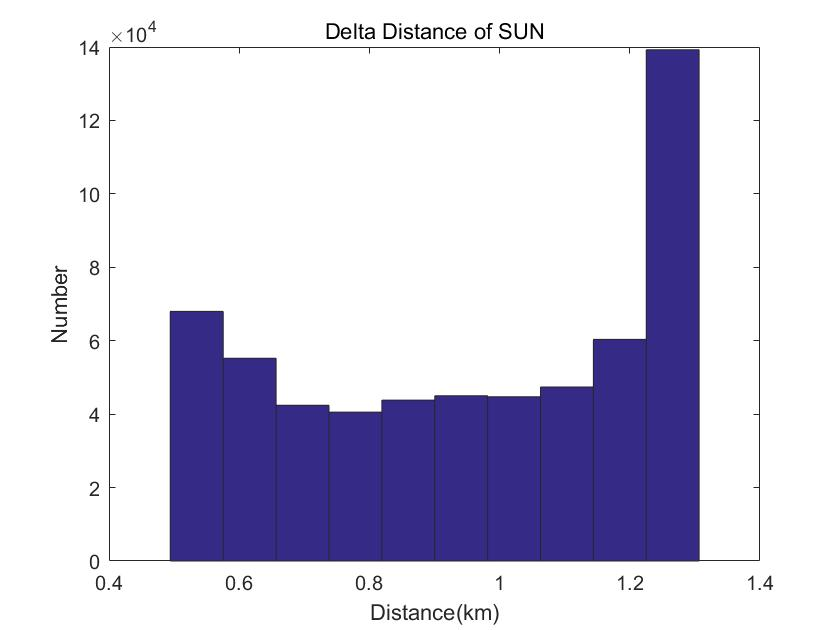
\includegraphics[width=0.6\textwidth]{figs/check_results/delta_distance_of_sun.png}
\caption{太阳距离的差异。}
\label{0411_check_results1}
\end{figure}

\begin{figure}
\centering
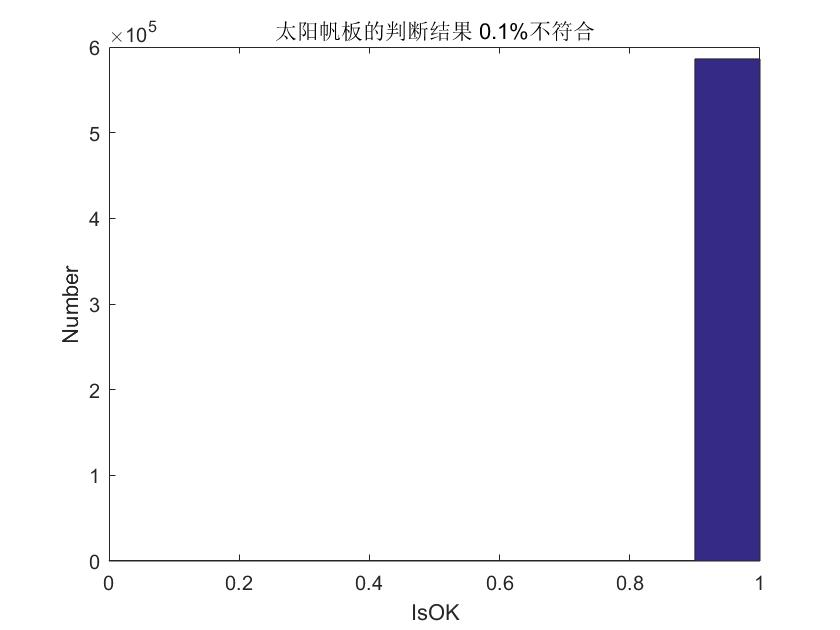
\includegraphics[width=0.6\textwidth]{figs/check_results/solar_panel_disagreement.png}
\caption{太阳帆板夹角的不符合率。}
\label{0411_check_results2}
\end{figure}

\begin{figure}
\centering
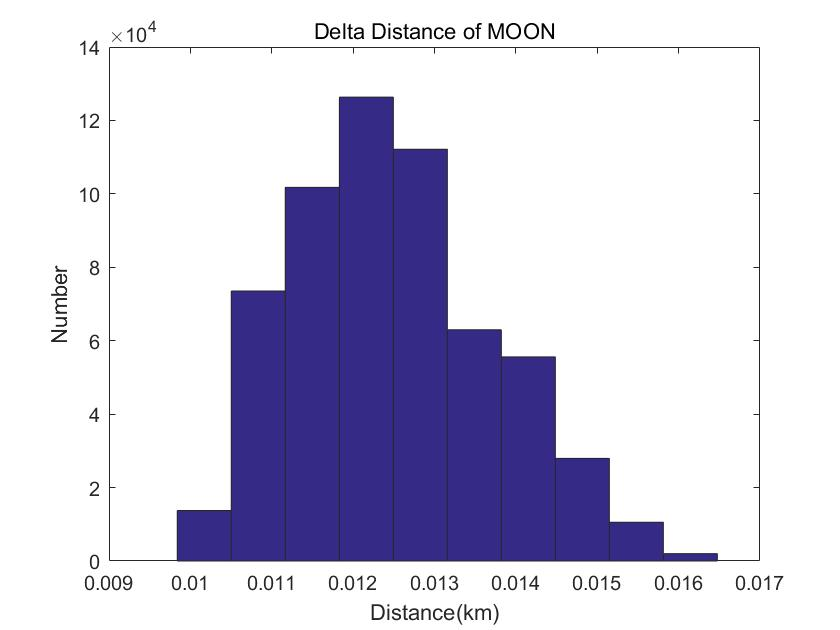
\includegraphics[width=0.6\textwidth]{figs/check_results/delta_distance_of_moon.png}
\caption{月球距离的差异。}
\label{0411_check_results3}
\end{figure}

\begin{figure}
\centering
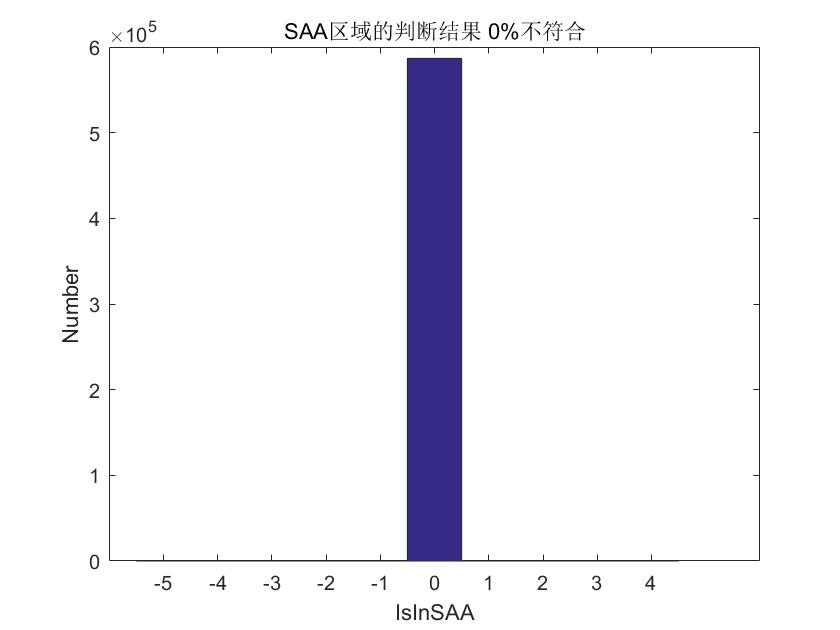
\includegraphics[width=0.6\textwidth]{figs/check_results/saa_disagreement.png}
\caption{SAA区域的不符合率。}
\label{0411_check_results4}
\end{figure}

\begin{figure}
\centering
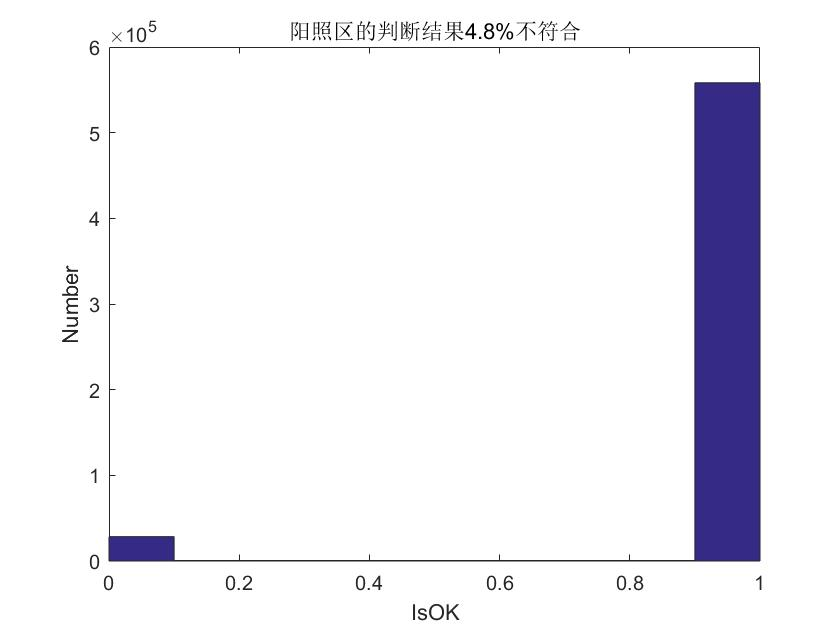
\includegraphics[width=0.6\textwidth]{figs/check_results/sunside_disagreement.png}
\caption{阳照区的不符合率。\RT{这个结果是初步判断结果,从中发现了张鑫的程序中bug,该bug已经修复。}}
\label{0411_check_results5}
\end{figure}
在这些检验结果中,阳照区的不符合率最大。将不符合的结果掉出来检查后发现,角度判断中出现的最大
差异可达30\textdegree,这明显是不正常的结果。后来与张鑫提及此事,他回忆到在最后输出结果的
部分曾经修改过一些代码:修改后的输出结果的第一列是曝光开始的时间,而阳照区的判断是在望远镜
转动到指定的天区之前进行的判断,因此会出现很大的差异。随后将阳照区判断进行更新后跑完模拟发现
结果就很正常了。因为模拟程序中所使用的阳照区判据还是比较粗糙的(将地球处的太阳光作了平行光近似,
另外未考虑大气折射效应,即蒙气差),所以在用唐怀金提供的新盘踞进行判断的时候,有$45\%$的结果
不符合~\footnote{根据唐怀金提供的判据,我用C++独立地重新实现了检验程序。}。
但是对这些不符合的结果仔细查看后发现,差异其实非常小,最大的差异也不超过1.5\textdegree,
并且这些差异的符号全部是负的,也就是说张鑫的结果中那些不符合唐怀金的判据的都是将本该在阳照区的
给“误判”成在阴影区了。这是一个合理的结果,因为按照张鑫的判据,阴影区的范围要略微大于唐怀金的
阴影区。至此,我们可以认为阳照区的判断是通过测试了,后期只需要稍微修改一下模拟代码中的相应
模块即可。

\begin{figure}
\centering
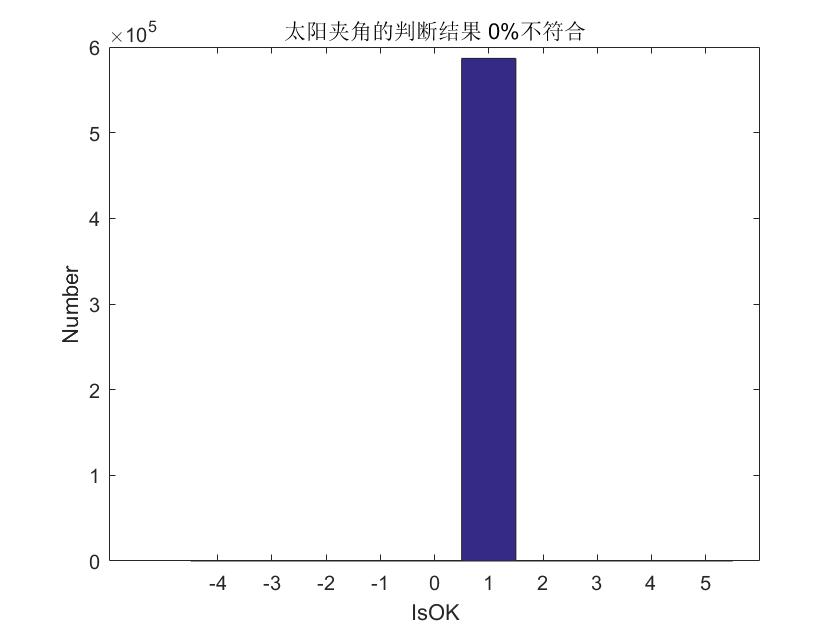
\includegraphics[width=0.6\textwidth]{figs/check_results/sun_angle_disagreement.png}
\caption{太阳夹角的不符合率。}
\label{0411_check_results6}
\end{figure}

\begin{figure}
\centering
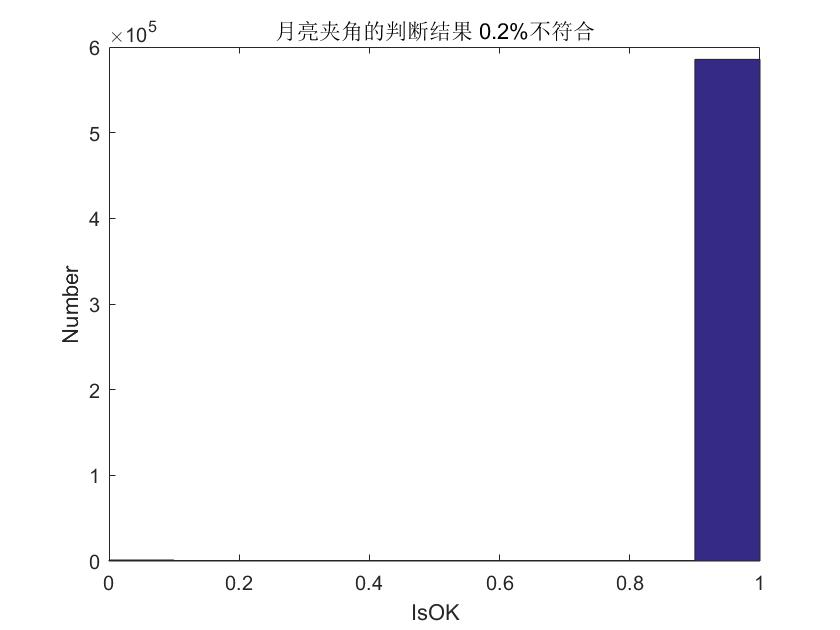
\includegraphics[width=0.6\textwidth]{figs/check_results/moon_angle_disagreement.png}
\caption{月球夹角的不符合率。}
\label{0411_check_results7}
\end{figure}

%==================================================================
\subsection{17日}
将发电效率公式中的$\cos^2$换成$\cos^4$之后重新跑了一遍模拟,结果发现能源条件还是不起作用,最终的
编排结果并没有出现什么不同。这TM就蛋疼了。。。

%==================================================================
\subsection{18日}
上午联系5院的孙国童,询问了一下性能衰减的那些系数具体该如何理解。对方回答说,这些百分比的系数在使用时
都是以相乘的方式计算的。

%==================================================================
\subsection{20日}
再次联系5院的孙国童,告之我们估算的结果显示并不会出现能源不平衡的问题。电话中孙提到,总的发电功率不会
超过13~$\text{kJ/s}$(???)。

%==================================================================
\subsection{23日}
与孙国童简要讨论了,可以用电池处的功率进行计算。由于“冗余设计”、“分流”、“驱动”等消耗,
电源输出端的功率不会超过$13~\text{kW}$。就目前的编排模拟需要来看,可以先简化充电、放电的过程。目前
我们的模拟与他们所给出的限制之间主要差异在望远镜机动时的处理方式上:他们考虑了机动时帆板法线与太阳夹角
改变的这个因素,而我们目前在模拟的过程中忽略了“机动”。\RT{\kaishu 另外,五院所给的限制暂时也没有进一步
考虑阳照区的范围受大气折射的影响。}

\BT{\kaishu 电话中询问了机动时的转动应该满足什么条件,孙国童的回答是需要保证不产生像旋。}

%%%%%%%%%%%%%%%%%%%%%%%%%%%%%%%%%%%%%%%%%%%%%%%%%%%%%%%%%%%%%%%%%%%
%%%%%%%%%%%%%%%%%%%%%%%%%%%%%%%%%%%%%%%%%%%%%%%%%%%%%%%%%%%%%%%%%%%
\section{5月}

%==================================================================
\subsection{9日}
测试坐标系旋转代码,以及根据旋转矩阵来确定旋转轴和旋转角度;根据旋转角度可进一步确定旋转所需的时间。
\RT{补充用于描述望远镜指向转动的数学表达式}


%==================================================================
\subsection{10日}
\RT{补充机动时的发电量计算的公式}

\MT{\heiti 机动时的最差发电情况可以假设为帆板法线与太阳连线的夹角为25\textdegree 。}

\BT{\kaishu 我关于程序的一些疑问:每一次寻找下一个目标天区时,在搜索到最佳的观测天区之前,望远镜的姿态
是什么样子的?是否有变量保存了望远镜上一次观测结束后的姿态信息?}

%==================================================================
\subsection{11日}
孙国童提了一个问题:如果在轨任务时,天地存在1秒时差\footnote{这里的“时差”是“注入文件里规定的某条指令的执行
时间”和实际在轨该条指令的执行时间的差异。就好比巡天序列里某一次观测开始时间,咱们在地面算的时候,按地面时钟
要求下周一中午12点,在轨运行时,按舱上时钟的12点执行,但天地时钟差了1秒,那么,相当于观测开始时间差了一秒。},
对观测会造成什么影响?

\MT{(14日)詹老师说运行指令是每周上传一次,延时对于巡天而言没有什么影响;但是对短时的天文现象会有影响。}

%==================================================================
\subsection{14日}
与孙国童沟通CMG建模的事情:
\begin{itemize}
\item “这个模型模型恐怕不好建,设计整个飞行器的热控;热控是CMG工作产生的,但是散热
靠整器的热控系统;这和当时的整舱温度条件、外热流、辐射器温度都密切相关”

\item “巡天效率方面,建议让长光优化杂散光抑制能力”

\item “上一轮优化工作,貌似只有平台作出了让步;现在CMG单机的压力确实特别大”

\item “机动,稳定,微震动,寿命,几乎所有指标都被压得没有余量,工程风险特别大”
\end{itemize}

%==================================================================
\subsection{21日}
\RT{需要学会合理安排任务,提高时间利用率!同时要克服“排斥”和“抵触”情绪!}

\subsection{22-25日}
这几天选取了不同面积的天区划分来进行编排模拟。这些模拟的一些重要模型假设和参数设置总结如下:
\begin{itemize}
\item 能源平衡的计算过程中,太阳能发电的效率与帆板法线和太阳
\end{itemize}


%==================================================================
\subsection{28日}
跑了两组运行模拟,主要参数设置如下:
\begin{itemize}
\item 运行时间为10年+105天;
\item 天区划分范围为$|b|>18$\textdegree,$|\delta|>19.5$\textdegree ;
\item $\beta=15$\textdegree ;
\item 优先观测的高纬度阈值分别为25\textdegree 和22.5\textdegree
\end{itemize}
预计的可观测面积为18019平方度。\footnote{\RT{这里预计的可观测面积是通过蒙特卡洛的方法估计得到的,存在约几十平方度
的误差。以下所提及的预计可观测面积都包含相似的随机误差。}}

这次模拟的结果未能完整输出到文件中去,因为在最后模拟快结束的时候,负责输出失败信息的部分存在一个bug。
但根据已经输出到文件的结果来看,在10年内是可以完成17500平方度的巡天任务的。

%==================================================================
\subsection{29日}
在fix那个导致输出异常的bug之后,重新跑了两组运行模拟,主要参数设置如下:
\begin{itemize}
\item 运行时间为10年+105天;
\item 天区划分范围为$|b|>18$\textdegree ,$|\delta|>18.5$\textdegree ;
\item $\beta=15$\textdegree ;
\item 优先观测的高纬度阈值分别为25\textdegree 和22.5\textdegree
\end{itemize}
预计的可观测面积为18532平方度。

根据前次的结果稍微做了一些调整,适当增加了天区划分的面积。最终模拟得到观测天区覆盖面积分别为
18528平方度和18454平方度,几乎完整覆盖了所划分的所有天区,验证了28日根据不完整的结果作出的推断。


%==================================================================
\subsection{30日}
调节$\beta$角使得可用于观测的面积所占10年的比例为$70\%$,此时的$\beta$角为10.25\textdegree,
但后来忘记修改主函数中的$\beta$角的设置了。

因为可观测时间增加了,于是又稍微增加了天区划分的面积,选取的参数为$|b|>16.5$\textdegree 和
$|\delta|>18$\textdegree,对应的预计可观测面积为19562平方度。

因为$\beta$角实际上并没有减少,所以最终模拟得到的天区覆盖面积并没有增加,反而有略微的减少。
具体数值分别为18361平方度和17773平方度。

\subsection{31日}
今早看到30日提交的运行模拟的结果之后菜突然意识到忘记修改程序中的$\beta$角设置了,悲催。。。
目前程序正在辛勤的劳动着,等等吧。。。

%====================
\section{6月}

\subsection{1日}
昨天重新提交的模拟已经完成,两个结果均达到了预期,并且给出了同样的观测天区面积,具体数值
结果为19562平方度。\MT{这次模拟中也发现了一些程序运行效率的问题。这次划分的天区面积实际上
有一些偏小,于是在模拟到达后期的时候,再也找不到可以观测的天区了,使得每一次循环都在进行
“空跑”,而且由于步长相对于正常模拟的时候要小很多,导致最后一段时间的模拟更加费时了。}

\subsection{2日}
昨天傍晚重新提交了两组模拟,再次增加了划分天区的面积,后来结果显示,10年内的观测面积可以
超过20000平方度。

\subsection{3日}
对天区搜索部分进行了简单的优化,利用一个int型指针数组来记录当前可观测天区的ID,并且每隔一段时间
进行一次更新,将那些已经观测过的(并且观测次数到达指定的次数)天区的ID从这个指针数组中去掉,从而
减少了每次搜索时的平均查找次数。当可观测天区的数目等于0的时候,模拟程序将会终止运行,不再像之前
那样出现“空跑”的情况了。

\subsection{\MT{4日}}

需要三组情况下的模拟结果:
\begin{itemize}
\item 没有$\beta$角限制的情况下,10年内最多可以观测多大面积的天区?(25000平方度是最低要求)
\item 在$\beta=15$\textdegree 的情况下,10年内最多可以观测多大面积的天区?(17500平方度是最低要求)
\item 在$\beta=10.25$\textdegree 时,观测时间占10年的$70\%$,此时可以观测的最大面积为多少?
\end{itemize}

以下是阶段性的结果,作为对以上3个问题的回答:
\begin{table}[htp]
\begin{center}
\vspace{0.2cm}
\begin{tabular}{|c|c|c|c|}
\hline
  & 无$\beta$角限制 & $\beta=15$\textdegree & $\beta=10.25$\textdegree \\
\hline
$\beta$角时间(年) & 无 & 2.5 & 1.9 \\
\hline
停靠总时间(年) & 1.4 & 1.1 & 1.1 \\
\hline
观测总时间(年) & 8.6 & 6.6 & 7.0 \\
\hline
观测总面积(平方度) & 25849 & 18528 & 20163 \\
\hline
\end{tabular}
\caption{\MT{截止6月3日所得到的一些结果。(注:其中无$\beta$角限制的结果是5月22日获得的,当时假设的
还是5次停靠;目前正在重新模拟4次停靠的情况;另外,在计算(可)观测总时间的时候,因为$\beta$角时间和
停靠时间会有部分重合,所以(可)观测总时间+$\beta$角时间+停靠总时间会略微大于10年)。}}
\end{center}
\label{tab:3results}
\end{table}

\subsection{6日}
通过在台式机上进行测试,发现了5日对代码进行的一些简化~\footnote{注释掉了部分代码片段,这些地方的判断
因为采取了动态减少搜索范围而变得不必要。}存在一些bug。因为不是每一步都要进行天区搜索范围的更新,因此有
很多时候,在SearchNewPoints内进行循环判断的时候,依然需要判断当前指向的天区是否已经被观测过了(出现
bug就是因为将这一部分的判断给注释掉了);之前没有发现这个bug的时候,这部分相应的代码被注释掉了,因此
原先被判定为“已经观测过的天区”再一次被当做候选的可观测天区了,从而导致实际模拟的天区覆盖面积偏小很多。

\subsection{7日}
今早台式机的最新结果显示,在不施加beta角限制的情况下,10年内的最大巡天覆盖面积可达到26197平方度,并且
此时还剩余了93天的时间未使用。目前在lens上正在运行的模拟是有beta限制的情况,增加了天区划分的面积,期待
可以达到21000平方度(之前20163平方度的结果显示最后剩余103天未使用)。

刚刚又提交了一个不施加beta角限制的模拟,进一步增加了天区划分的面积,预计可以观测26800平方度。同时在
台式机上也运行着一个同样的模拟,明早应该就可以看到结果了。

\subsection{8日}
最新结果:
\begin{itemize}
\item 不施加beta角限制的情况下,10年内的最大观测面积现在可以达到26815平方度(剩余15天未使用,
可以压榨的空间已经所剩无几了)
\item 控制beta角($\beta=10.25$\textdegree)所占时间和停靠所占时间为总时间的$30\%$的前提下,最大
巡天覆盖面积可以达到21734平方度,几乎刚刚好用完10年时间。
\end{itemize}

以下是最新结果
\begin{table}[htp]
\begin{center}
\caption{\MT{截止6月8日所得到的一些结果。}}
\vspace{0.2cm}
\begin{tabular}{|c|c|c|c|}
\hline
  & 无$\beta$角限制 & $\beta=15$\textdegree & $\beta=10.25$\textdegree \\
\hline
$\beta$角时间(年) & 无 & 2.5 & 1.9 \\
\hline
停靠总时间(年) & 1.4 & 1.1 & 1.1 \\
\hline
观测总时间(年) & 8.6 & 6.6 & 7.0 \\
\hline
观测总面积(平方度) & \RT{26815} & 18528 & \RT{21734} \\
\hline
\end{tabular}
\end{center}
\label{tab:3results}
\end{table}

\subsection{18日}
继续尝试增大天区划分的面积,在没有$\beta$角限制的情况下可以看到多大的巡天面积:
\begin{itemize}
\item 在银纬10\textdegree 和黄纬10.5\textdegree 的情况下,巡天所能达到的面积为27409平方度(预计27542平方度)
\item 在银纬10\textdegree 和黄纬11.5\textdegree 的情况下,巡天所能达到的面积为26539平方度(预计26933平方度)
\end{itemize}

\subsection{20日}
提交了一组(7种不同天区面积划分)编排模拟,每一模拟划分的银纬、黄纬范围以及模拟结果在下面
的表~\ref{tab:0620}中给出:
\begin{table}
    \centering
    \renewcommand{\arraystretch}{1.15}
    \begin{tabular}{ccccrl}
        \toprule
        银纬($b$)     & 黄纬($B$)        & 巡天面积 & 巡天时间 & 模拟运行所花费时间 & 划分/未观测天区数\\
        \cmidrule(r){1-1} \cmidrule(lr){2-2} \cmidrule(lr){3-3} \cmidrule(lr){4-4} \cmidrule(lr){5-5}  \cmidrule(lr){6-6} 
        10.0 \textdegree  & 11.5 \textdegree & 26854 & 10.222 yr & 102439 sec / 28.46 hr & 814732 / 0\\
        10.0 \textdegree  & 11.0 \textdegree & \RT{27187} & 10.262 yr &   95454 sec / 26.52 hr & 824860 / 0\\
        10.0 \textdegree  & 10.5 \textdegree & \RT{27409} & 10.285 yr & 90817 sec / 25.23 hr & 831621 / 0\\
        10.0 \textdegree  & 10.0 \textdegree & \RT{27404} & 10.286 yr &  89158 sec / 24.77 hr & 841775 / 2403 \\
        10.0 \textdegree  & 9.5   \textdegree & \RT{27370} & 10.286 yr &  88878 sec / 24.69 hr & 851947 / 6088 \\
        10.0 \textdegree  & 9.0  \textdegree &  \RT{27063} & 10.286 yr &  92239 sec / 25.62 hr & 862143 / 12179 \\
        9.5  \textdegree  & 11.0 \textdegree & \RT{27419} & 10.286 yr & 91864 sec / 25.52 hr & 833981 / 340\\
        9.5  \textdegree  & 10.5 \textdegree & \RT{27415} & 10.286 yr & 94017 sec / 26.12 hr & 840794 / 1936\\
        9.5  \textdegree  & 10.0 \textdegree & \RT{27358} & 10.286 yr & 88864 sec / 24.68 hr & 851024 / 5962\\
        9.0  \textdegree  & 10.5 \textdegree & \RT{27355} & 10.286 yr & 91429 sec / 25.40 hr & 850025 / 5678\\
        9.0  \textdegree  & 10.0 \textdegree & \RT{27106} & 10.286 yr & 92873 sec / 25.80 hr & 860331 / 10988\\
        8.5  \textdegree  & 10.0 \textdegree & 26807 & 10.286 yr & 90930 sec / 25.25 hr & 869613 / 17868\\
        8.5  \textdegree  & 9.50 \textdegree & 26812 & 10.286 yr & 90356 sec / 25.10 hr & 880020 / 25271\\
        8.0  \textdegree  & 9.50 \textdegree & 26896 & 10.286 yr & 91869 sec / 25.52 hr & 889422 / 32283\\
        8.0  \textdegree  & 9.00 \textdegree & 27050 & 10.286 yr & 90024 sec / 25.00 hr & 899920 / 39589\\
        \bottomrule
    \end{tabular}
    \caption{通过不断的尝试来找出最大的巡天面积(这9(11)组模拟均使用了12个CPU核心,主频为2792.87MHz)。
    \MT{又提交了(9.5\textdegree ,11\textdegree )和(9.5\textdegree ,10\textdegree )两组模拟。}
    (\RT{该表最新结果填写于6月24日。})}
    \label{tab:0620}
\end{table}

\subsection{21日}
开始密集地搜索最大可观测天区面积、以及具体的划分方式(但是还没有开始进行策略的优化)。
新增4组不同天区划分的模拟:
\begin{itemize}
\item (10\textdegree,11\textdegree)
\item (10\textdegree,10\textdegree)
\item (10\textdegree,9.5\textdegree)
\item (10\textdegree,9\textdegree)
\end{itemize}

\subsection{22日}
收到詹老师的邮件,需要几组模拟更新两页PPT的图。这次需要的模拟是假设$70\%$的时间用于巡天观测($\beta=10.25$\textdegree)。
另外的一些变化是更改了部分极深度巡天的区域,先将这些区域的天球坐标总结在表~\ref{tab:ultra_deep_areas}中。另外,
稍微调整了极深度巡天区域的大小,原来设定的角直径为8.1\textdegree,现在改为8\textdegree。

\begin{table}
  \centering
  \renewcommand{\arraystretch}{1.15}
  \begin{tabular}{cccc}
      \toprule
      区域  & 赤道(deg) & 黄道(deg) & 银道(deg) \\
      \cmidrule{1-1} \cmidrule{2-2} \cmidrule{3-3} \cmidrule{4-4}
      ELAIS S1 & & 345.97, -43.18 & 312.57, -72.55 \\
      XMM-LSS & & 31.04, -17.90 & 170.58, -59.36 \\
      Extended Chandra Deep Field-South & & 40.29, -45.47 & \\
      COSMOS & & 150.70, -9.39 & \\
      GOODS-S & & 41.13, -45.19 & 223.57, -54.44 \\
      GOODS-N & & 148.36, 57.29 & 125.89, 54.83 \\
      Extended Groth Strip (EGS) & & 179.96, 60.26 & 96.48, 59.60 \\
      Ultra Deep Survey (USD) & & 0.21, -5.54 & 96.83, -65.73 \\
      银心 & & 266.85, -5.59 & 0,0\\
      反银心 & & 77.50, 6.09 & 180,0\\
      A & & 230, 50 & \\
      B & & 310, -60 & \\
      \bottomrule
  \end{tabular}
  \caption{从网上找到的坐标基本都是
   赤道坐标系下的数值,需要转换到黄道和银道坐标系下,但是发现会有细微的差异。我所使用的坐标转换工具为:
  \url{https://lambda.gsfc.nasa.gov/toolbox/tb_coordconv.cfm}。}
  \label{tab:ultra_deep_areas}
\end{table}

24日下午3点左右,三组模拟完成,模拟结果在表~\ref{tab:0623_results}中给出:
\begin{table}
    \centering
    \renewcommand{\arraystretch}{1.2}
    \begin{tabular}{ccccrl}
        \toprule
        银纬($b$ deg)     & 黄纬($B$ deg)        & 巡天面积 & 巡天时间 & 模拟运行所花费时间 & 划分/未观测天区数\\
        \cmidrule(r){1-1} \cmidrule(lr){2-2} \cmidrule(lr){3-3} \cmidrule(lr){4-4} \cmidrule(lr){5-5}  \cmidrule(lr){6-6} 
        \RT{15.0} & \RT{13.5} & \bm{\RT{22068}} & 10.286 yr & 68018 sec / 18.89 hr & 690892 / 6220 \\
        \RT{15.0} & \RT{13.0} & 21904 & 10.286 yr & 68091 sec / 18.91 hr & 700230 / 12922 \\
        \RT{15.0} & \RT{12.5} & 21700 & 10.286 yr & 68941 sec / 19.15 hr & 709550 / 19670 \\
        \RT{15.0} & \RT{12.0} & 21495 & 10.286 yr & 70285 sec / 19.52 hr & 715766 / 24670 \\
        \GT{15.0} & \GT{11.5} & \bf{\GT{21116}} & 10.286 yr & 72142 sec / 20.04 hr & 725098 / 32679 \\
        \GT{14.0} & \GT{11.5} & 20596 & 10.286 yr & 71998 sec / 20.00 hr & 742779 / 46943 \\
        \GT{13.0} & \GT{11.5} & 20048 & 10.268 yr & 73537 sec / 20.43 hr & 760601 / 62737 \\
        \bottomrule
    \end{tabular}
    \caption{在$\beta=10.25$\textdegree 的情况下,10年(实际使用的轨道数据时间未10.286年)内有$70\%$的时间可以用于巡天。}
    \label{tab:0623_results}
\end{table}

\subsection{24日}
